\documentclass{article}[10pt]
%%%%%%%%%%%%%%%%%%%%%%%%%%%%%%%%%%%%%%%%%%%%%%%%%%%%%%%%%%%%%%%%%%%%%%%%
%%%%%%%%%%%%%%%%%%%%%%%%%%%%%%%%%%%%%%%%%%%%%%%%%%%%%%%%%%%%%%%%%%%%%%%%
%%%%%%%%%%%%%%%%%%%%%%%%%                   %%%%%%%%%%%%%%%%%%%%%%%%%%%%
%%%%%%%%%%%%%%%%%%%%%%%%%    MATHSYMBOLS    %%%%%%%%%%%%%%%%%%%%%%%%%%%%
%%%%%%%%%%%%%%%%%%%%%%%%%                   %%%%%%%%%%%%%%%%%%%%%%%%%%%%
%%%%%%%%%%%%%%%%%%%%%%%%%%%%%%%%%%%%%%%%%%%%%%%%%%%%%%%%%%%%%%%%%%%%%%%%
%%%%%%%%%%%%%%%%%%%%%%%%%%%%%%%%%%%%%%%%%%%%%%%%%%%%%%%%%%%%%%%%%%%%%%%%
\newcommand{\tr}{{\rm tr}}
\newcommand{\hf}{\frac{1}{2}}

\newcommand{\field}[1]{\mathbb{#1}}					    
\newcommand{\CC}{{\field C}}
\newcommand{\RR}{{\field R}}
\newcommand{\ZZ}{{\field Z}}
\newcommand{\al}{\alpha}
\newcommand{\pr}{^{\prime}}
\newcommand{\xt}{\xi_{2}}   
\newcommand{\Q}{\bar{Q}}
\newcommand{\la}{\mathcal{L}}
\newcommand{\mcL}{\mathcal{L}}
\newcommand{\bt}{\mathbf{\theta}}
\newcommand{\bd}{\mathbf{d}}
\newcommand{\Ns}{N_{\mathrm{sample}}}
\newcommand{\Nt}{N_{\mathrm{total}}}
\newcommand{\MM}[1]{\mathcal{M}_{#1}}
\newcommand{\p}{\Phi}
\newcommand{\ld}{\cal{D}}
\newcommand{\half}{\frac{1}{2}}
\newcommand{\fdelJ}{\f{\delta}{\delta J}}
\newcommand{\bea}{\begin{eqnarray}}
\newcommand{\eea}{\end{eqnarray}}
\newcommand{\Man}[1]{$\mathfrak{#1}$}
\newcommand{\man}[1]{\mathfrak{#1}}
\newcommand{\del}{\partial}


\newcommand{\be}{\begin{equation}}
\newcommand{\ee}{\end{equation}}
\newcommand{\beqn}{\begin{eqnarray}}
\newcommand{\eeqn}{\end{eqnarray}}


\newcommand{\dbcolor}{white}

\newcommand{\apj}{ApJ}
\newcommand{\prd}{Phys.Rev.D.}
\newcommand{\mnras}{MNRAS}
\newcommand{\jcap}{JCAP}
\newcommand{\nat}{Nature}
\newcommand{\physrep}{Physics Reports}

%%%%%%%%% Fonts
\usepackage{amsfonts}
\usepackage{amsmath}
\usepackage{amsmath,amssymb}
\usepackage{verbatim}
\usepackage{fancyvrb}
\usepackage{moreverb}
\usepackage{cprotect}
%%%%%%%%%font color
\usepackage{color}
\usepackage[colorlinks=true]{hyperref}
%%%%%%%%% Graphics
\usepackage{graphicx}
\usepackage{subfigure}
%\usepackage{epsf}
%%%%%%%%% layout tools
\usepackage{setspace}
\usepackage{lscape}
\usepackage{changepage}
\usepackage{longtable}
\usepackage[table]{xcolor}% http://ctan.org/pkg/xcolor
%\usepackage[table]{xcolor}% http://ctan.org/pkg/xcolor
%\usepackage[dvips]{color}


\usepackage{graphicx}
\newcommand{\thetalctrue}{\theta^{SN_{\rm{true}}}}
\begin{document}
\section{Objectives}
The objectives for this document are to
\begin{itemize}
\item Have a description of the models, assumptions and detailed description of the mathematical formulae used. 
\item Explore similar, but slightly different models and methods to analyze them\end{itemize} 

\section{Model 1}
This is the model discussed in the first hack and described in Fig.~\ref{fig:model1} 
\begin{figure}[h]
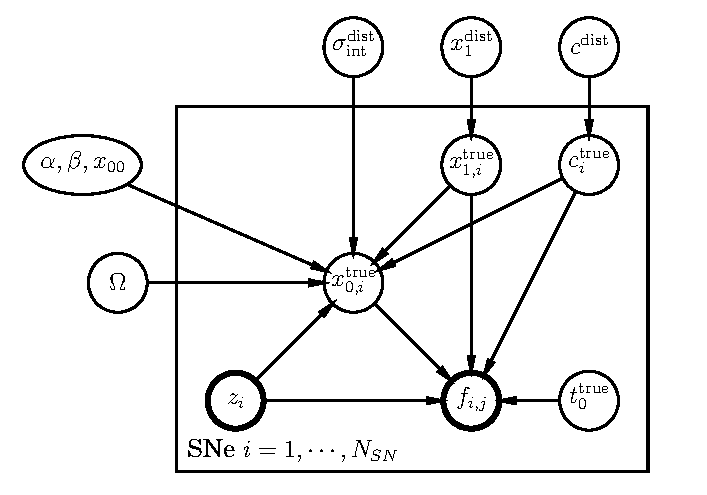
\includegraphics{images/snpgm}
\caption{Model 1}
\label{fig:model1}
\end{figure}

\subsection{Observed Values}
There are three different quantities that are assumed to be observed values or 
`data' in the Bayesian sense.
\begin{itemize}
\item Cosmological redshift of each supernova, with $z_i$ denoting the redshift of the ith supernova.
\item Observed flux of i'th supernova in the j'th epoch with the associated bandpass, denoted by $f_{i,j}$.
\item The noise in each of the measurements of flux, which is due to noise in the number of photons from
the supernova-source, sky background as well as due to efficiency in image differencing. In this model, we will assume that this is totally due to the sky background which is measured independently, and perfectly. We will denote this by 
$\sigma^{sky}_{i,j}$ where, $i$ indexes the supernova, while $j$ indexes the epoch of observation of the supernova. 
\end{itemize}

\subsection{The Model}
This discussion is based on the `SALT2' model, with certain assumptions or 
interpretations beyond the exact model. 

The SALT2 model has two parts:
\begin{itemize}
    \item A light curve model with parameters $\{t_0, x_0, x_1, c, z\}.$ The model also has a likelihood for the flux values at different times:
        $P(f_{i,j} \vert \{t_0, x_0, x_1, c, z\}, \{\sigma_{i,j}\} )$
    \item A Tripp ansatz that relates the peak absolute magnitude $M_{b}$ in the rest frame BessellB band to the parameters ${x_1, c}$ and a global parameter $M$. 
    \be
    M_b = M + \beta c - \alpha x_1
    \ee
    so that the peak magnitude $m_B^{\star}$ in Bessell B band calculated from
    the model is related as
    \be
    \mu = m_B^{\star} - M_b = m_B^{\star} + \alpha x_1 - \beta c - M
    \ee
    where
    \be
    m_B^{\star} = -2.5 \log_{10}{(f_B^{\star})}, \quad f_B^{\star} = \int d\lambda T(\lambda) \frac{d S}{d\lambda}(\lambda, p=0)
    \ee
    which is related mostly to $x_0,$ since the contribution from terms 
    involving $c$ and $x_1$ to this quantity is constrained to be exactly $0$
    in defining the SALT2 model at $p=0$ at the central wavelength of the 
    BessellB band. In this very good approximation, $m_B^{\star} = -2.5 \log_{10}{(x_0)} -2.5 \log_{10}{(F_0)},$ where $F_0$ is a constant which can be evaluated for the SALT2 model. Thus, we will treat $x_0$ and $m_B^{\star}$ as equivalent quantities. Further, abusing our notation, we will redefine:
    \be
    m_b^{\star} = - 2.5 \log_{10}{(x_0)} , \qquad M \rightarrow M + 2.5\log_{10}{(F_0)}
    \ee
\end{itemize}
As an additional ingredient, we will be using is the interpretation of intrinsic
dispersion:
\begin{itemize}
 
    \item It is well known that standardization in the above manner is not complete, and the distance moduli derived using the above equations have residual scatter. There is some evidence that this scatter is different in different bands, and therefore cannot be completely modelled by a scatter in $M$ above, but we shall ignore this for now and model this by assuming that 
        \be M \sim \mathcal{N}(M_0, \sigma_{int}) \ee  
where $\sigma_{int}$ is the intrinsic dispersion which we will infer from 
the study.
Thus, the true properties of a particular supernova is completely specified by the set of parameters $\thetalctrue = \{x_0/m_B^{\star}, x_1, c, t_0\}$
\end{itemize}
Combining these, we can obtain the probability distributions
$ P(m_B^{\star}\vert \Omega, M_0, z, x_1, c)$ or equivalently $P(x_0 \vert \Omega, M_0, \sigma_{int}, x_1, c, z)$:
\beqn
P(m_B^{\star} \vert \Omega, M_0, z, x_1, c, \sigma_{int} ) &=& 
\int dM P(m_B^{\star} \vert M, \Omega, \alpha, \beta, x_1, c)P(M \vert M_0, \sigma_{int}) \\
&=&
P(\mathcal{N}(\mu(\Omega, z) - \alpha x_1 + \beta c + M_0, \sigma_{int}^2) 
\eeqn
While, we are assuming that 
\be
P(x_1 , c \vert \Omega, M_0, z, \sigma_{int}) = P(x_1, c) = P(x_1) P(c) 
\ee
which we may relax in other models. In this model,  we have
\beqn
P(\thetalctrue \vert \Omega, \alpha, \beta, z, M_0, \sigma_{int}) &\equiv& P(m_B^{\star} \vert x_1, c, t_0, \Omega, z, \alpha, \beta, M_0, \sigma_{int}) \nonumber \\
&\times& P(x_1, c, t_0, z, \Omega, \alpha, \beta, M_0, \sigma_{int})\\
&=& P(m_B^{\star} \vert x_1, c, M_0, \sigma_{int}, \Omega, z, \alpha, \beta) \\
&\times& P(x_1, c, t_0 ,\sigma_{int}) P(\Omega, z, \alpha, \beta) \nonumber\\
&=& \mathcal{N}(\mu(\Omega, z) - \alpha x_1 + \beta c + M_0, \sigma^{int}) \\
&\times&  P(x_1, c, t_0 ,\sigma_{int}) P(\Omega, z, \alpha, \beta)  
\eeqn

\subsection{Posterior Samples of the Cosmology}
The quantity we are interested in is the posterior distribution of the cosmological parameters $\Omega$ (where we will use $\Omega$ to denote the set of
cosmological parameters, given the set of measurements $f_{i, j}$ , $\sigma_{i,j}$ which is 
\be
P(\Omega \vert \{f_{i,j}, \sigma_{i,j}, z_i,  \}) = 
        \int d\alpha d\beta d\sigma_{int}d M_0 P(\Omega, \alpha, \beta, M_0, \sigma_{int} \vert \{f_{i,j}, \sigma_{i,j}, z_i\})
\ee
We would like to do this integral by drawing samples from the space of cosmological parameters $\Omega, \alpha, \beta, M_0, \sigma_{int}$ with their frequencies
according to above probability distribution. This requires evaluating
$
P(\Omega, \alpha, \beta, M_0, \sigma_{int} \vert \{ f_{i,j}, \sigma_{i,j}, z_i\}) 
,$ at least, upto a constant of proportionality. We try to evaluate this using
samples of individual light curve parameters inferred without any prior on 
cosmology.
\be
P(\Omega, \alpha, \beta, \sigma_{int}, M_0 \vert \{ f_{i,j}, \sigma_{i,j}, z_i\}) 
    \propto P(\{ f_{i,j}\} \vert \Omega, \alpha, \beta, M_0, \sigma_{int}, \{\sigma_{i,j}, z_i \} ) P(\Omega, \alpha, \beta, M_0, \sigma_{int}) 
\ee
To get the RHS, we need 
\beqn
 P(\{f_{i,j}\} \vert \Omega, \alpha, \beta, \sigma_{int}, M_0, \{\sigma_{i,j},z_{i}\}) &=& \int  \prod_{i} d\thetalctrue_{i} P(\{f_{i,j} \}, \vert \{\sigma_{i,j}, \thetalctrue_i, z_i \}) \\
  &\times& P(\{\thetalctrue_i \}\vert \Omega, \alpha, \beta, \sigma_{int}, M_0, z_i) \nonumber\\ 
 &=& \prod_i \int d\thetalctrue_i  P(\{f_{i,j} \}, \vert \{\sigma_{i,j} , z_i, \thetalctrue_i, z_i \})\\
 %P(\{\thetalctrue_i \}\vert \Omega, \alpha, \beta, z_i)
 &\times& P({t_0}_i)  P({x_1}_i) P(c_i)  \mathcal{N}(\mu(\Omega, z) - \alpha {x_1}_i + \beta c_i + M_0, \sigma^{int})  \\
 &=& \prod_i \left( \int d\thetalctrue_i \Phi_i (\thetalctrue_i) w_i (\thetalctrue_i)\right) \\
 &=& \prod_i I_i
\eeqn
where  $\Phi_i(\thetalctrue_i)$ is proportional to the posterior distribution of the model parameters $\thetalctrue_i$ of i'th supernova  
\be 
\Phi_i(\thetalctrue_i) \equiv P(\{f_{i,j} \}, \vert \{\sigma_{i,j} , z_i, \thetalctrue_i, z_i \})P(t_{0})P(x_1)P(m_B^{\star})P(c)
\ee
and therefore $w_i(\thetalctrue_i)$ are given by  
\be
w_i = \mathcal{N}(\mu(\Omega, z) - \alpha {x_1}_i + \beta c_i + M_0, \sigma^{int}) / P(m_B^{\star})
\ee
Using the equal weight samples (indexed by $j$) of posteriors of light curve model parameters obtained from the individual light curves, we can do the individual integrals $I_i$ for each 
supernova
\be
I_i \approx \frac{1}{N_i} \sum_j \thetalctrue_{i,j} w_i ( \thetalctrue_{i,j}) 
\ee
where $N_i$ is the number of samples of light curve model parameters of the 
$j'\rm{th}$ supernova.
The first term is the posterior distribution of the light curves parameters 
found separately in a previous stage. The integral in the last equation for each SN is then a sum over samples indexed by $j$ 
\be
\sum_j \thetalctrue_j w(\thetalctrue_j) 
\ee
\end{document}
